\documentclass{iosart2c}
%\usepackage{makeidx}  % allows for indexgeneration
\usepackage{graphicx}
\usepackage{caption}
\usepackage{subcaption}
\usepackage[hidelinks]{hyperref}
%\usepackage{hyperref}
%\usepackage[utf8]{inputenc}
%\usepackage{moreverb}
\usepackage{listings}
%\usepackage{float}
%\usepackage{graphicx}
\usepackage{adjustbox}
%\usepackage{caption}
%\usepackage{subcaption}
\usepackage{xcolor}
%\usepackage{wrapfig}
%\usepackage{algorithm}
%\usepackage{algorithmic}
%\usepackage{amssymb}
%\usepackage{amsmath}
%\usepackage{tikz}
%\usetikzlibrary{shapes}
%\usepackage{subfig}
\usepackage{pifont}
\usepackage{todonotes}
\usepackage{microtype}
\newcommand{\xmark}{\ding{55}}%
\newcommand{\cmark}{\ding{51}}%
\usepackage{colortbl}
%\usepackage{times}
\definecolor{gray}{gray}{0.8}
\definecolor{LightCyan}{rgb}{0.8,1,1}
%\usepackage{todonotes}
\usepackage{comment}
\usepackage{multirow}
\usepackage{textcomp}
\usepackage{booktabs}
\usepackage{comment}
\newcommand{\ntextnumero}{{\fontfamily{txr}\selectfont \textnumero}}
\usepackage{tikz}
\usetikzlibrary{shapes,arrows,positioning,fit,backgrounds}
\newcommand{\hsp}{\vphantom{Ag}}

\renewcommand*\ttdefault{cmtt}

\usepackage{chngcntr}
\AtBeginDocument{\counterwithout{lstlisting}{chapter}}

\lstset{ %
  basicstyle=\footnotesize\sf,        
  tabsize=2, columns=flexible
}

\usepackage{hyperref}
\hypersetup{
    colorlinks, linkcolor={black},
    citecolor={black}, urlcolor={black},
    pdftitle={LSQ: The Linked SPARQL Queries Dataset},    % title
    pdfauthor={Muhammad Saleem, Muhammad Intizar Ali, Aidan Hogan, Qaiser Mehmood, Axel-Cyrille Ngonga Ngomo},     % author
    pdfsubject={International Semantic Web Conference},   % subject of the document
    pdfkeywords={SPARQL;} {endpoints;} {Linked Data;} {queries;} {LSQ}, % list of keywords
}

\begin{document}

\begin{figure}[float]
\centering
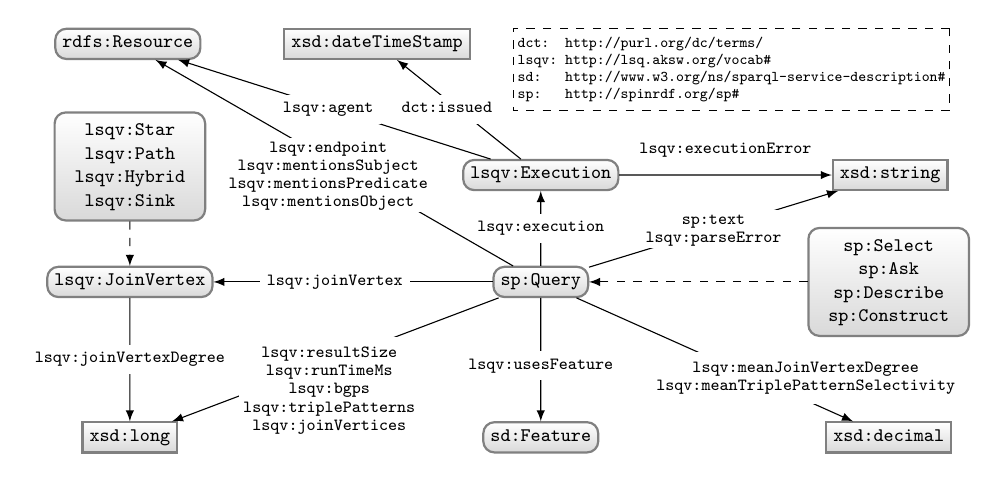
\begin{tikzpicture}[scale=0.77, every node/.style={transform shape}]

\tikzset{
	iri/.style={
		draw=black!50!white, 
		rectangle,
           	rounded corners,
           	thick,
           	text centered,
		top color=white, 
		bottom color=black!15, 
		font=\tt\small\hsp},
	lit/.style={
		draw=black!50!white, 
		rectangle,
		thick,
		text centered,
		top color=white, 
		bottom color=black!15, 
		font=\tt\small\hsp},
	arrout/.style={
		->,
		-latex,
		font=\tt\footnotesize\hsp},
	arrin/.style={
           	<-,
           	latex-,
		font=\tt\footnotesize\hsp}
}

\node[iri,anchor=center,] (q) {sp:Query};

\node[iri,anchor=center,right=4.4cm of q.center] (t) {\begin{tabular}{c}sp:Select\\sp:Ask\\sp:Describe\\sp:Construct\end{tabular}}
  edge[arrout,dashed] node[auto] {} (q);
  
\node[lit,anchor=center,below=2.3cm of t.center] (dec)
{xsd:decimal}
   edge[arrin] node[fill=white,xshift=1.5cm,yshift=-0.3cm] {\begin{tabular}{@{}c@{}}lsqv:meanJoinVertexDegree\\[-0.3ex]lsqv:meanTriplePatternSelectivity\end{tabular}} (q);


\node[iri,anchor=center,above=1.5cm of q.center] (e) {lsqv:Execution}
   edge[arrin] node[fill=white] {lsqv:execution} (q);

\node[lit,anchor=center,above=1.9cm of e.center,xshift=-2.7cm] (dts) {xsd:dateTimeStamp}
   edge[arrin] node[fill=white,xshift=-0.2cm] {dct:issued} (e);

\node[iri,anchor=center,left=2.9cm of dts.center] (res) {rdfs:Resource}
   edge[arrin] node[fill=white,outer sep=0ex, inner sep=0ex,yshift=-0.2cm,xshift=-0.1cm] {\begin{tabular}{@{}c@{}}lsqv:endpoint\\[-0.3ex]lsqv:mentionsSubject\\[-0.3ex]lsqv:mentionsPredicate\\[-0.3ex]lsqv:mentionsObject\end{tabular}} (q)
   edge[arrin] node[fill=white,xshift=-0.1cm] {lsqv:agent} (e);

\node[lit,anchor=center,right=4.8cm of e.center] (str) {xsd:string}
    edge[arrin] node[fill=white,above,yshift=0.28cm,inner sep=0ex] {lsqv:executionError} (e)
    edge[arrin] node[fill=white,inner sep=0ex,outer sep=0ex] {\begin{tabular}{@{}c@{}}sp:text \\[-0.3ex] lsqv:parseError\end{tabular}} (q);
    
\node[iri,anchor=center,left=5.4cm of q.center] (jv) {lsqv:JoinVertex}
   edge[arrin] node[fill=white,xshift=-0.3cm] {lsqv:joinVertex} (q);
   
\node[lit,anchor=center,below=2.3cm of jv.center] (long) {xsd:long}
   edge[arrin] node[fill=white,yshift=-0.5cm,xshift=-0.1cm] {\begin{tabular}{@{$\!$}c@{$\!$}}lsqv:resultSize\\[-0.3ex]lsqv:runTimeMs\\[-0.3ex]lsqv:bgps\\[-0.3ex]lsqv:triplePatterns\\[-0.3ex]lsqv:joinVertices\end{tabular}} (q)
   edge[arrin] node[fill=white] {lsqv:joinVertexDegree} (jv);
   
\node[iri,anchor=center,above=1cm of jv.center] (t) {\begin{tabular}{c}lsqv:Star\\lsqv:Path\\lsqv:Hybrid\\lsqv:Sink\end{tabular}}
  edge[arrout,dashed] node[auto] {} (jv);
  
\node[iri,anchor=center,below=2.3cm of q.center] (f) {sd:Feature}
    edge[arrin] node[fill=white,yshift=-0.1cm] {lsqv:usesFeature} (q);  
  
\node[right=0.7cm of dts.north east,anchor=north west,font=\scriptsize\tt,dashed,draw] (pre)
{\begin{tabular}{@{$\!$}l@{~}l@{$\!$}} %
dct: & http://purl.org/dc/terms/\\
lsqv: & http://lsq.aksw.org/vocab\#\\ %
sd: & http://www.w3.org/ns/sparql-service-description\#\\ %
sp: & http://spinrdf.org/sp\# %
\end{tabular}};
\end{tikzpicture}
\caption{LSQ data model (dashed lines indicate sub-classes)}
\label{fig:Schema}
\end{figure}
\end{document}